\documentclass[12pt,]{article}


%%-------------------------------------------------
%% Various packages
%%-------------------------------------------------
\usepackage{booktabs} % for stuff like \bottomrule in tables
\usepackage{changepage} % for \adjustwidth
\usepackage{float} % to float tables
\usepackage[left=1in,top=1in,right=1in,bottom=1in]{geometry} % sets the document margins
\usepackage{adjustbox} % for \resizebox for tables
\usepackage{dcolumn} % to align on the decimal point of numbers in table columns
\usepackage{bm} % to make math symbols bold with \bm{}
\usepackage{lmodern} % font
\usepackage{amsmath} % maths



%%-------------------------------------------------
%% Sections, subsections, subsubsections, paragraphs
%%-------------------------------------------------

\setcounter{secnumdepth}{5} 
% This line sets the section counting level to 5, meaning section, subsection, subsubsection, paragraph and subparagraph are numbered. You can't set it higher -- 5 is the maximum section levels available in markdown


\usepackage[compact]{titlesec} % needed for the \filcenter command below

% Change the section commands so that they look like I want them too
\makeatletter
\renewcommand\section{\@startsection {section}{1}{\z@} 
                                   {-3.5ex \@plus -1ex \@minus -.2ex}
                                   {2.3ex \@plus.2ex}
                                   {\large\bfseries\filcenter}} % everything from the standard article.cls; I just customized the last line
\renewcommand\subsection{\@startsection{subsection}{2}{\z@}%
                                     {-3.25ex\@plus -1ex \@minus -.2ex}
                                     {1.5ex \@plus .2ex}
                                     {\normalsize\bfseries}} % same here
\renewcommand\subsubsection{\@startsection{subsubsection}{3}{\z@}
                                     {-3.25ex\@plus -1ex \@minus -.2ex}
                                     {1.5ex \@plus .2ex}
                                     {\normalsize\itshape}} % same here
\renewcommand\paragraph{\@startsection{paragraph}{4}{\z@}
                                    {-3.25ex \@plus -1ex \@minus -.2ex}
                                    {1.5ex \@plus .2ex}
                                    {\normalsize}} % for paragraph, I changed the three last lines, as I want paragraph to be indented, with \newline afterwards etc. just like sections
\makeatother

% Note: I couldn't use \titleformat{\section} etc. here because that doesn't play nicely with paragraph. More precisely, it needs several other lines and twists which were too complicated to figure out


% I want the paper titles as sections, because I want them to be part of the toc. I want the numbering to start with the subsection, but I don't want "1.1" -- I want the subsection to start with "1". The following two lines achieve that:
\renewcommand{\thesection}{{}}
\renewcommand{\thesubsection}{\arabic{subsection}} 



%%-------------------------------------------------
%% Abstract
%%-------------------------------------------------

\usepackage{abstract}




%%-------------------------------------------------
%% Graphics/Plots
%%-------------------------------------------------
\usepackage{graphicx}
% Generate all images so they have a width \maxwidth. This means
% that they will get their normal width if they fit onto the page, but
% are scaled down if they would overflow the margins.
\makeatletter
\def\maxwidth{\ifdim\Gin@nat@width>\linewidth\linewidth
\else\Gin@nat@width\fi}
\makeatother
\let\Oldincludegraphics\includegraphics
\renewcommand{\includegraphics}[1]{\Oldincludegraphics[width=\maxwidth]{#1}}

% Make all figures use 'H' position by default:
\makeatletter
\def\fps@figure{H}
\makeatother



%%-------------------------------------------------
%% Listings/Hyperrefs
%%-------------------------------------------------
\newtheorem{hypothesis}{Hypothesis}
\usepackage{setspace}
\makeatletter
\@ifpackageloaded{hyperref}{}{%
\ifxetex
  \usepackage[setpagesize=false, % page size defined by xetex
              unicode=false, % unicode breaks when used with xetex
              xetex]{hyperref}
\else
  \usepackage[unicode=true]{hyperref}
\fi
}
\@ifpackageloaded{color}{
    \PassOptionsToPackage{usenames,dvipsnames}{color}
}{%
    \usepackage[usenames,dvipsnames]{color}
}
\makeatother
\hypersetup{breaklinks=true,
            bookmarks=true,
            pdfauthor={Simon Heuberger (Department of Government)},
             pdfkeywords = {},  
            pdftitle={PhD Dissertation Prospectus: Advances in Public Opinion Measurement Using Modern Statistical Methods:
Sequential Blocking, Mode Effects, and the Power of Moral Arguments},
            colorlinks=true,
            citecolor=blue,
            urlcolor=blue,
            linkcolor=blue,
            pdfborder={0 0 0}}
\urlstyle{same}  % don't use monospace font for urls


%%-------------------------------------------------
%% Header-includes
%%-------------------------------------------------



%%-------------------------------------------------
%% Bib/Natbib
%%-------------------------------------------------
\usepackage{natbib}
\bibliographystyle{apalike}




%%-------------------------------------------------
%% For flowchart(s)
%%-------------------------------------------------

\usepackage{tikz}
\usetikzlibrary{shapes,arrows,positioning}

% Define block
\tikzstyle{block} = [rectangle, draw, fill=blue!20, text width=1cm, text centered, rounded corners, minimum height=3em]

% Define another block
\tikzstyle{block2} = [rectangle, draw, fill=blue!20, text width=2cm, text centered, rounded corners, minimum height=3em]

% Define yet another block
\tikzstyle{block3} = [rectangle, draw, fill=blue!20, text width=3cm, text centered, rounded corners, minimum height=3em]

% And another block
\tikzstyle{block4} = [rectangle, draw, text width=3cm, text centered, rounded corners, minimum height=3em]

% Define cloud
\tikzstyle{cloud} = [draw, ellipse, fill=red!20, node distance=1cm, minimum height=3em]

% Define another cloud
\tikzstyle{cloud2} = [draw, ellipse, node distance=1cm, minimum height=3em]

% Define line
\tikzstyle{line} = [draw, -latex', node distance = 0.1cm, auto]


%%-------------------------------------------------
%% For math
%%-------------------------------------------------

% next 11 lines to create math symbol "reallywidehat"
\usepackage{scalerel,stackengine}
\stackMath
\newcommand\reallywidehat[1]{%
\savestack{\tmpbox}{\stretchto{%
  \scaleto{%
    \scalerel*[\widthof{\ensuremath{#1}}]{\kern-.6pt\bigwedge\kern-.6pt}%
    {\rule[-\textheight/2]{1ex}{\textheight}}%WIDTH-LIMITED BIG WEDGE
  }{\textheight}% 
}{0.5ex}}%
\stackon[1pt]{#1}{\tmpbox}%
}



%%-------------------------------------------------
%%-------------------------------------------------
%% Actually begin document
%%-------------------------------------------------
%%-------------------------------------------------



\begin{document}



%%-------------------------------------------------
%% Title & Subtitle
%%-------------------------------------------------

\pagenumbering{gobble} % suppresses page numbering until I start it for the text body

{\begin{center}
{\Large\fontfamily{ptm}\selectfont \scshape{{PhD Dissertation Prospectus}}}
\vskip 30pt
{\Large \doublespacing Advances in Public Opinion Measurement Using Modern Statistical Methods:
Sequential Blocking, Mode Effects, and the Power of Moral Arguments}
\vskip 30pt
\end{center}}




%%-------------------------------------------------
%% Author, Address, Date & Email
%%-------------------------------------------------


{\begin{center}
\textbf{Simon Heuberger} \vskip 0.1pt Department of Government   
	
American University

\vskip 30pt

{\itshape{9 August 2018}}

 
\end{center}}

\clearpage



%%-------------------------------------------------
%% Abstract (latex default: single-spaced)
%%-------------------------------------------------
\begin{abstract}
\vspace{-0.1cm} \noindent \small I am writing a methods dissertation that proposes advances in public
opinion measurement with modern statistical methods. Particularly, these
advances consist of new methods for ordinal survey measures. The
dissertation consists of three papers, where two make quantitative
methods contributions and one applies both contributions in a
substantive analysis in American Politics.\newline Paper I improves
balance in survey experiments by providing a new method of sequential
blocking for ordinal covariates. In political science, the most common
ordinal covariates are income and education. Both are highly important
predictors of public opinion and behavior. It is currently not possible
to block on ordinal covariates. I develop a software tool to make this
method freely available to other researchers. The tool can be applied to
in-person and online survey experiments, as it includes code that
provides a finished web-based questionnaire interface. I demonstrate the
benefits of my method with simulations, external data, and original
data.\newline Paper II provides a measurement for mode differences in
surveys. While there is an abundance of studies that analyze mode
differences, existing research can only pinpoint certain parts of
surveys where respondents' reasctions are and are not affected by mode,
the literature offers little help in identifying whether systematic mode
effects exist that affect the distributions of responses and the survey
instrument as a whole. I develop a measure of entropy that addresses
this shortcoming, as traditional statistical approaches used to
investigate these differences are not suitable. I test this measure with
external and original data and locate its results within the enviroment
of the Total Survey Error (TSE).\newline Paper III uses both
methodological contributions from papers I and II and investigates
whether moral arguments are part of what makes a political frame strong.
First, I conduct a meta-analysis of previous experimental framing
studies. Second, I conduct an online poll that tests strong frames from
previous experimental studies on their moral content. Third, I conduct a
second online poll to gain qualitative insights about how people define
moral arguments. Fourth, I design frames with moral and amoral arguments
to complement gaps in previous experiments and test these frames in a
third online poll. Finally, I design a questionnaire for an online and
face-to-face survey experiment that assesses the effect of moral and
amoral frames. All polls and the online version of the survey experiment
are fielded on MTurk. The face-to-face version of the survey experiment
is fielded for an undergraduate population at American University. The
sequential blocking method for ordinal covariates developed in paper I
is applied when both versions of the experiment are fielded. The ordinal
entropy measure developed in paper II is applied in the subsequent
analysis of both versions' experimental results. The substantive results
show whether moral arguments form a part of what makes a political frame
strong.
    \par
\end{abstract}

\clearpage



%%-------------------------------------------------
%% Table of contents
%%-------------------------------------------------


{
\hypersetup{linkcolor=black}
\setcounter{tocdepth}{4}
\tableofcontents
}


\clearpage


%%-------------------------------------------------
%% Text body
%%-------------------------------------------------

\pagenumbering{arabic} % starts page numbering here

\noindent \doublespacing \hypertarget{paper-i-improving-balance-in-survey-experiments-with-ordinal-variables}{\section{Paper
I: Improving Balance in Survey Experiments with Ordinal
Variables}\label{paper-i-improving-balance-in-survey-experiments-with-ordinal-variables}}

\addtocontents{toc}{\protect\addvspace{8pt}}

\subsection{Introduction}\label{seq-intro}

Survey experiments collect background information and contain questions
that represent differing types of treatment, depending on the specific
nature of the experiment. Such experiments are created to uncover any
effect of a certain treatment on public opinion and behavior. In order
to uncover such potential effects, treatment groups need to be
comparable. All treatment groups need to look the same in every measure,
i.e.~they must be balanced. This can be achieved through random
assignment of participants to treatment groups. One such option for
random assignment is complete randomization. For each participant, the
computer flips a coin to decide which treatment group to assign her to
\citep{urdan_statistics_2010}. Using complete randomization for large
samples results in balance based on the Law of Large Numbers. Using it
for small samples, however, can result in serious imbalance. It can
easily be that the treatment groups will not look the same. This can
leave experimental results in statistically murky waters
\citep{imai_quantitative_2018, king_designing_1994, fox_applied_2015}.
In survey experiments, the overall sample size is often split across
several treatment groups. \citet{chong_framing_2007}, for instance,
split 869 participants in a framing experiment on urban growth over 17
treatment groups, which leads to an average of just over 50 participants
per group. Complete randomization is very unlikely to lead to balanced
treatment groups of this size. Researchers need to employ statistical
methods to obtain balanced groups here.

One statistical method to ensure balance for small samples is blocking.
Blocking involves the arrangement of participants in groups that are
similar to one another in terms of the participants' covariates,
i.e.~their background information. Within these groups, participants are
then randomly assigned. This is different from complete randomization,
where participants are immediately randomly assigned without taking
their covariate information into account.

To apply blocking, a researcher needs to know all the covariate
information for all participants before assigning treatment. Oftentimes,
however, this is not possible as participants arrive for assignment at
differing times. The researcher knows the covariate information of the
arriving participant and (if she is not the first one) of the previous
already assigned participants, but she does not have any information
about future incoming participants. She thus needs more advanced
statistical methods to block these participants. One such method is
sequential blocking. Sequential blocking assigns each participant based
on information from previously assigned participants and the incoming
participant herself, while participants are still arriving to be
assigned. Sequential blocking uses statistical methods to `decide' which
group to assign a participant to. These measurements differ depending on
the form that the covariate information comes in. Some covariate
information is binary (e.g.~gender) while other is categorical
(e.g.~party ID, race), to name only two. Research has shown that
sequential blocking greatly improves balance in small samples
\citep{moore_blocking_2013}.

While sequential blocking is possible for a variety of variable forms,
there is currently no method to sequentially block on ordinal variables,
such as income and education. Substantively, this means that a
researcher currently cannot block incoming participants based on their
provided level of education and income. This is problematic for
political science, as education and income represent two of the
strongest predictors of political behavior. I develop a new method of
sequential blocking for ordinal variables that fills this gap. This
method is freely available to other researchers as a package using the
open-source software R. The R package provides functions that allow
researchers to apply sequential blocking for ordinal variables in both
in-person and online survey experiments. Substantively, I employ this
method in simulated data, external data from political science
experiments published in peer-reviewed journal articles, and original
data in the form of an online and face-to-face survey experiment on the
importance of moral arguments in political framing. The following
sections provide background on sequential blocking and complete
randomization, showcase the statistical development of the new ordinal
sequential blocking method, and give more detail about the data to be
used with this method.

\subsection{Theory}\label{seq-theory}

\subsubsection{Preliminary Notations on
Randomization}\label{seq-notations}

The simplest of experiments has two potential outcomes for participants
\(i\): \(y_{1i}\) and \(y_{0i}\), with 1 denoting the treatment and 0
referring to the control. If a researcher, for example, intends to
analyze the effect of a 2-week mathematic training camp on high school
students' performance in exams, she devises an experiment where one half
of her student sample participates in the camp (treatment) and the other
half abstains (control). At the end of the camp, both groups take the
same exam. If both groups of students look the same regarding their
covariates (age, mathematic skill, intelligence etc.), a comparison of
the groups' average test results reveals the Average Treatment Effect
(ATE):

\singlespacing

\vspace{-0.5cm}

\[\beta_i = y_{1i} - y_{0i}\]

\doublespacing

More specifically, for a sample of \(n\) students, this comparison
reveals the Sample Average Treatment Effect (SATE):

\singlespacing

\vspace{-0.5cm}

\[\frac{1}{n} \sum\limits_{i=1}^n y_{1i} - y_{0i}\]

\doublespacing

A central characteristic of such a comparison is the fundamental problem
of causal inference
\citep{holland_1986_statistics, rubin_1974_estimating}: We are unable to
observe both potential outcomes for the same participant at once. In our
case, we cannot observe how well student A performs in the exam after
participating in the camp whilst also observing how well the same
student A would have performed without taking part in the camp. If we
could, it would be simple to calculate the True Average Treatment Effect
(TATE) \citep{moore_2012_multivariate}:

\singlespacing

\vspace{-0.5cm}

\[\overline{TE} = \frac{1}{2n} \sum\limits_{i=1}^{2n} (y_{1i} - y_{0i})\]

\doublespacing 

Since the TATE is unobservable, we need to use statistical means to
assess the counterfactuals. This can be done by balancing the treatment
and control groups. If both groups of students look the same in every
measure, we can use the students who participated in the camp
(treatment) to estimate what would have happened to the students who did
not participate (control) if the abstaining students had in fact
attended the camp. The crucial aspect is of course whether the two
groups do indeed look the same in terms of the students' covariates.
There are two main mechanisms by which this can be achieved: Complete
randomization and blocking.

\subsubsection{Complete Randomization and Blocking}\label{seq-complete}

Complete randomization is equivalent to flipping a coin for each
participant to be assigned to treatment or control. This chance
procedure gives each participant an equal chance of being assigned to
either group (or groups, in case of multiple treatment groups)
\citep{lachin_1988_properties}. Complete randomization increases
covariate balance as \(n\) increases \citep{imai_2009_essential}. The
larger a researcher's sample, the better the resulting balance from
complete randomization. Complete randomization enables the comparison of
the SATE to be free from systematic error, which allows the researcher
to attribute any treatment effects to the treatment
\citep{king_a-politically_2007}.

While complete randomization thus guarantees balance as the sample size
reaches infinity, it often does not do so in the naturally finite sample
sizes researchers actually work with. With huge samples, the Law of
Large Numbers predicts that treatment groups `selected' through complete
randomization will be balanced. With small samples, however, it is
possible to get `unlucky' and end up with unbalanced groups
\citep{imai_2008_misunderstandings}. Blocking can help achieve balance
in such scenarios \citep{epstein_2002_rules}.

Blocking involves the arrangement of participants in groups that are
similar to one another in terms of the participants' covariates. As
mentioned above, the key aspect in experimental studies is whether the
treatment and control groups look the same. In complete randomization,
this is achieved by random chance. In blocking, this is achieved by
using covariate information about the participants. Researchers use
observed covariates to create similar treatment and control groups
before treatment is assigned. Blocking is thus better suited to
achieving balance in finite samples, as it ``directly controls the
estimation error due to differing levels of observed covariates in the
treatment and control groups'' \citep[p.~463]{moore_2012_multivariate}.

Efficient blocking focuses on covariates that affect the outcome. In
U.S. politics, for instance, it is widely established that party ID
represents one of the major driving forces behind public opinion
\citep{abramowitz_disappearing_2010, druckman_how_2013, fiorina_culture_2011, king_polarization_1997}.
Making sure that participants in treatment and control groups have
identical levels of party ID is thus crucial in experiments that test
the effect of interventions on public opinion.

\subsubsection{Blocking v. Post-Experiment OLS Controls}\label{seq-ols}

Researchers often employ complete randomization in survey experiments
and control for covariates post-hoc in OLS regression models. This is
done to increase balance and model precision. Proponents of this
approach might question the need for blocking approaches if post-hoc OLS
controls can achieve similar balance and are much less computationally
and mathematically complex. While controlling for covariates undoubtedly
improves balance over `basic' complete randomization, it does not
achieve the level of balance that blocking can provide. Most crucially,
this is because any OLS model requires assumptions about the choice of
controls to include. More often than not, it is very difficult if not
impossible to determine all needed controls. Such assumptions are not
required in blocked experiments. Additionally, blocking balances
variation, which post-hoc controls cannot provide. Finally, it stands to
reason that ex-ante balance prior to treatment is preferable to post-hoc
adjustments as it removes the possibility for errors to be introduced.

\subsubsection{Sequential Blocking}\label{seq-sequential}

Sequential blocking is a special form of blocking. Generally, there are
two main starting positions for the researcher who wants to conduct an
experiment: (1) The researcher knows all covariate information of all
participants at the time of randomization, and (2) covariate information
of participants `trickles in' as the experiment progresses and
participants arrive for assignment. Complete randomization,
i.e.~flipping a coin for each participant to be assigned to treatment or
control, is possible in both positions. `Normal', or for our purposes
`nonsequential', blocking can only be used in scenario 1: The researcher
possesses all information about all participants when the experiment
begins. Sequential blocking, on the other hand, is applied when the
researcher does not know all covariate information of all participants
when the experiment begins. Instead, she only possesses the covariate
information of the current incoming participant and previously assigned
participants, but not future incoming participants. This is scenario 2.
Sequential blocking is thus blocking `on the go'.

When all participant characteristics are known when the experiment
begins (scenario 1), sequential blocking is not necessary, as no
participants arrive individually for treatment. In many political
experiments, researchers have an already-collected data set in front of
them at the start of the experiment and then randomize a set of
households, precincts, or individuals to treatments all at once. All
covariate information on all participants is known, i.e.~the
characteristics of all participants are known at the time of
randomization. Examples are any studies that use pre-existing databases.
A prominent example are the American National Election Studies (ANES)
that are often used to analyze voter turnout \citep[see for
instance][]{jackman_2018_does, leighley_who_2014}.

In these experiments, `nonsequential' blocking suffices to create
homogeneous groups within which treatments can be assigned. In an
experiment of scenario 2, however, the researcher has much less
information about the eventual full sample to use in assigning treatment
than in an experiment with pre-existing data sets. More advanced
statistical methods are thus required to exploit available background
information to block `on the go', i.e.~to block sequentially.
\citet{chow_2007_adaptive} identify four types of sequential
experiments, which are shown in Table \ref{seq-seq-designs}.

\begin{table}[H]
\caption{Different Randomization Designs For Sequential Experiments}
\centering
\resizebox{\textwidth}{!}{
\begin{tabular}{>{\itshape}l l}
\bottomrule 
\midrule
Non-Adaptive & Assignment probabilities (AP) fixed throughout the trial\\
Treatment-Adaptive & AP change based on numbers of participants already in treatment groups\\
Response-Adaptive & AP change as a function of previous participants' outcomes\\
Covariate-Adaptive & AP change based on previous participants and the current participant\\
\bottomrule
\multicolumn{2}{l}{\footnotesize{Adapted from Chow and Chang (2007)}} \\
\end{tabular}}
\label{seq-seq-designs}
\end{table}

Non-adaptive randomization and treatment-adaptive randomization can (and
often do) ignore the researcher's detailed data on participants. They
thus leave important information lying on the table. Response-adaptive
randomization varies probabilities based on knowledge about previous
participants' outcomes. This is likely very useful for clinical trials,
where one outcome is often the clear goal: Consider a test where the
treatment group receives an experimental medication to fight cancer and
the control group receives a placebo. If it becomes clear as the trial
progresses that the medication is effective in fighting cancer, it makes
sense to assign more people to treatment, as this could potentially save
their lives. In political science, this is not the case. Assessing
whether a certain survey treatment affects participants' support for a
political issue is not a matter of life and death. This leaves
covariate-adaptive randomization (CAR), which varies probabilities based
on knowledge about previous participants and the current participant,
which appears ideally suited.

\paragraph{Basic Covariate-Adaptive Randomization (CAR)
Approaches}\label{seq-car-basic}

There are two traditional approaches to covariate-adaptive randomization
(CAR). The first approach is the biased coin design developed by
\citet{efron_1971_forcing}, which sets the current participant's
treatment assignment probability using its entire covariate profile at
once. I follow Chow and Chang's brief and excellent description of
Efron's design \citep{chow_2007_adaptive} here:

\singlespacing

\vspace{-0.5cm}

\begin{equation*}
  P(\delta_j \lvert \Delta_{j-1}) = 
  \begin{cases}
    0.5 & \text{if $N_A(j) = N_B(j)$},\\
    \text{$p$} & \text{if $N_A(j) < N_B(j)$}, \\
    1 - \text{$p$} & \text{if $N_A(j) > N_B(j)$}.
  \end{cases}
\end{equation*}

\doublespacing

\(\delta_j\) is a binary indicator for treatment assignment of the
\(j\)th participant (\(\delta_j=1\) for treatment A; \(\delta_j=0\) for
treatment B).
\(\Delta_{j-1} = \left\{ \delta_1, ..., \delta_{j-1} \right\}\) is the
the cumulative set of treatment assignment up to participant \(j-1\).
Imbalance is measured by

\singlespacing

\vspace{-0.5cm}

\[\lvert D_n \rvert = \lvert N_A(n) - n \rvert.\]

\doublespacing

The second approach is minimization, developed by
\citet{pocock_1975_sequential}, which considers covariates one at a time
and can limit marginal imbalance across an arbitrarily large set of
covariates. I follow Rosenberger and Lachin's overview of the method
here \citep{rosenberger_2002_randomization}: Let
\(N_{ijk}(n), i = 1, ..., I, j = 1, ..., n_i, k = 1,2\) (1 = treatment
A, 2 = treatment B), be the number of participants in category \(j\) of
covariate \(i\) on treatment \(k\) after \(n\) participants have been
randomized. Suppose the (\(n + 1\))th participant to be randomized is a
member of categories \(r_1, ..., r_I\) of covariates \(1, ..., I\). Let
\(D_i(n) = N_{ir_{i}1}(n) - N_{ir_{i}2}(n)\), with the weighted
difference measure being \(D(n) = \sum\limits_{i=1}^I w_iD_i(n)\).
\(w_i\) are weights the researcher chooses based in the perceived
importance of covariates. If \(D(n)\) is lower than 0, then the weighted
difference measure indicates that treatment B was chosen more often so
far for that set, \(r_1, ..., r_I\), of strata, and that participant
\(n + 1\) should be assigned with higher probability to treatment A.
This argument holds vice versa if \(D(n)\) is greater than 0. According
to Pocock and Simon, the coin should be biased with

\singlespacing

\vspace{-0.5cm}

\[p = \frac{c^* + 1}{3} \]

\doublespacing

and the following rules implemented: If \(D(n) < 0\), assign the next
incoming participant to treatment A with probability \(p\). If
\(D(n) > 0\), assign the next incoming participant to treatment A with
probability \(1-p\). Finally, if \(D(n) = 0\), assign the next incoming
participant to treatment A with probability 1/2, where
\(c^* \in [1/2,1]\).

The biased coin and minimization approaches use discrete covariates with
a very small number of levels \citep{moore_blocking_2013}. Discrete
covariates allow for simpler pairing procedures, as the number of
possible covariate levels is finite. This is not the case for continuous
covariates, where the number of possible covariate levels rises
exponentially. Blocking on continuous covariates is thus not possible
with these traditional approaches
\citep{markaryan_2010_exact, rosenberger_2002_randomization, eisele_1995_biased}.

\paragraph{Extended CAR for Continuous Covariates}\label{seq-car-md}

In the standard approaches, the incoming participant is assigned to the
treatment group with the fewest participants with identical covariate
information. With continuous covariates, no two participants will look
the same, and thus identical participants do not exist.
\citet{moore_blocking_2013} develop a method to include continuous
variables in sequential blocking with CAR by exploiting relationships
between the current participant's covariate profile and those of all
previously assigned participants.

\citet{moore_blocking_2013} define the similarity between participants
with the Mahalanobis distance (MD) between participants \(q\) and \(r\)
with covariate vectors \(\bm{x}_q\) and \(\bm{x}_r\):
\newline \noindent \(MD_{qr} = \sqrt{(\bm{x}_q - \bm{x}_r)' \reallywidehat{\sum}^{-1} (\bm{x}_q - \bm{x}_r)}\).
To aggregate pairwise similarity, they implement the mean, median, and
trimmed mean of the pairwise MDs between the current participant and the
participants in each treatment condition: Participants are indexed with
treatment condition \(t\) using \(r \in \{1,...,R\}\). For each
condition \(t\), an average MD between the current participant, \(q\),
and the participants previously assigned, \(t\). If the distance in
terms of MD for the incoming participant is 2 in the control and 5 for
the treatment condition, the incoming participant looks more similar to
the control condition. To set the probability of assignment,
\citet{moore_blocking_2013} test several methods, most notably a set of
strategies that calculates the mean Mahalanobis distances for each
incoming participant, \(q\), for all treatment conditions, \(t\), and
sorts the treatment conditions by these averages. Randomization is
biased towards conditions with high scores. For each value of \(k\),
with \(k \in \{2,3,...,6\}\), the condition with the highest average MD
is then assigned a probability \(k\) times larger than all other
assignment probabilities, \(T-1\).

\paragraph{Extended CAR for Ordinal Covariates}\label{seq-car-ordinal}

\citet{moore_blocking_2013} extend basic blocking approaches to provide
a method to apply sequential blocking to continuous covariates. They
show that their approach significantly improves balance for some
experiments. I extend blocking approaches further by developing a method
to sequentially block on ordinal covariates. My method also extends
blocking methodology to previously unused multi-category treatments.

Consider the following simple example for a common ordinal variable in
political science: Income. Income is a strong predictor for political
behavior such as turnout, representation, or donations
\citep{dawood_campaign_2015, fiorina_disconnect_2009, leighley_who_2014}.
A researcher conducts a basic experiment with one treatment and one
control group. The researcher also collects information about income on
three levels: Low, medium, and high. For all already-assigned
participants, let the income distributions across these three levels
look like figure \ref{OrdIntEx} for both groups.

\begin{figure}
\centering
\includegraphics{prospectus_files/figure-latex/Plot_Ordinal_Income_Example-1.pdf}
\caption{Example Distributions of 3-Level Income in Treatment and
Control Groups\label{OrdIntEx}}
\end{figure}

A new participant arrives with low income. We need a suitable measure,
or measures, to define the dissimilarity between this incoming
participant and the already assigned participants. It would be easy to
transform these income levels into the numeric values of 1, 2, and 3,
and simply apply the Mahalanobis distance used for continuous variables.
In doing so, however, we would assume that the distance between 1 and 2
is the same as the distance between 2 and 3. We do not have to make such
a strong assumption if we keep the ordinal levels low, medium, and high.
Similarly, we could transform low, medium, and high income into three
dummy variables. Income would then look like non-ordinal variables such
as race or gender. Again, crucial information would be lost. We cannot
employ the mean because there is no mean for ordinal variables. Exact
matching, and with that Coarsened Exact Matching
\citep{iacus_2011_causal}, might suggest itself, since income is not a
continuous variable. Unlike matching, however, we are not looking to
create identical pairs of participants. We are comparing one participant
with one specific level of income with the whole distribution of income
across many other, previously-assigned participants. The distribution
rarely has one specific level, therefore there will not be exact matches
for the majority of incoming participants. In order to exploit the
unique information contained in ordinal variables, we need different
measures.

I propose a weighted approach that incorporates all levels of the
respective ordinal variable in question. Using only the incoming
participant's income level of the distribution for comparison would
ignore all the available information on the two other income levels,
medium and high, in all treatment groups, and treat income as a
one-level variable, thereby removing its very nature of an ordinal
variable. I propose to develop the following algorithm: Let an ordinal
variable have levels \(m_i = m_1, m_2, ..., m_I\). Let the level of an
incoming participant be \(m_1\). Let the number of treatment groups be
\(t_j = t_1, t_2, ..., t_J\), where \(J\) can take on any number to
account for binary and multi-category treatments. For each treatment
group, we calculate the proportion of participants with level \(m_1\),
\(p(m_1)\), and weight this proportion by \(\frac{I}{J+1}\). For each
treatment group, we then calculate the proportions of participants in
the next level \(m_2\), \(p(m_2)\), and weight this proportion by
\(\frac{I-1}{J+1}\). This is continued until the proportion of
participants for the last level \(m_I\), \(p(m_I)\), which is weighted
by \(\frac{1}{J+1}\). This gives us \(S_j\), the weighted average of the
income distribution for each treatment group:

\singlespacing

\vspace{-0.4cm}

\[S_j = \frac{I}{J+1} \times p(m_1) + \frac{I-1}{J+1} \times p(m_2) + \frac{I-2}{J+1} \times p(m_3) + ... + \frac{1}{J+1} \times p(m_I)\]

\vspace{0.1cm}

\doublespacing

Note that the proportions over all the treatment groups sum up to one,
\(\sum\limits_{i=1}^I p(m_I) = 1\). Note also that the sum of all
weights equals \(\frac{I}{2} \times (I+1)\). The numerators for the
respective level proportions are set in descending order because
\(m_1\), as the ordinal variable level of the incoming participant, is
the most important in the distribution, followed by \(m_2\), then
\(m_3\), and so on. Since we are adding up weighted proportions, a
higher weighted average \(S_j\) represents more similarity to the
incoming participant. She will thus be assigned to the treatment group
with the lowest \(S_j\).

In the simple income example given above, the income variable has three
levels, thus \(I=3\) (Low, Medium, and High Income), and there are two
treatment groups, thus \(J = 2\). The incoming participant has low
income, thus \(m_1 = \text{Low}\). In the control group,
\(p(\text{Low}) =\) 0.4, \(p(\text{Medium}) =\) 0.4, and
\(p(\text{High}) =\) 0.2. \(S_1\) for the control group thus is:

\[S_{\text{Control}} = \frac{3}{2+1} \times 0.4+ \frac{2}{2+1} \times 0.4 + \frac{1}{2+1} \times 0.2 = 0.733\]

In the treatment group, \(p(\text{Low}) =\) 0.3, \(p(\text{Medium}) =\)
0.1, and \(p(\text{High}) =\) 0.6. \(S_2\) for the treatment group thus
is:

\[S_{\text{Treatment}} = \frac{3}{2+1} \times 0.3 + \frac{2}{2+1} \times 0.1 + \frac{1}{2+1} \times 0.6 = 0.567\]

We thus assign the incoming participant with low income to the treatment
group.

\subsubsection{Computational Development}\label{seq-computational}

\paragraph{R Package: BlockExperiments}\label{seq-computational-r}

The new sequential blocking method I develop is built in R and made
freely available to other researchers as the R package
\texttt{BlockExperiments}. \texttt{BlockExperiments} includes the
functions provided by \texttt{blockTools} \citep{moore_2016_package} and
further improves on the state of the art. By incorporating
\texttt{blockTools}, \texttt{BlockExperiments} thus allows the user to
apply sequential blocking to binary, continuous, and ordinal variables.
It also includes web-components that allow the user to create a finished
web-based survey questionnaire that can be directly fielded online.
\texttt{BlockExperiments} can thus be employed for in-person sequential
survey experiments as well as online sequential survey experiments.

Figure \ref{in-person-workflow} shows a sample workflow for the use of
\texttt{BlockExperiments} in in-person experiments. Processes performed
by the software in R are shown as blue boxes. Actions that need to be
completed by the user outside of R are shown as red clouds.

\vspace{0.4cm}

\begin{figure}[H]
\centering
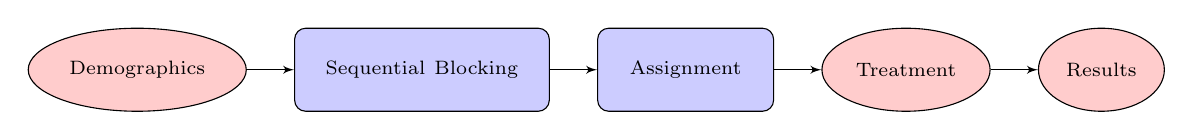
\begin{tikzpicture}
    \node [block3]  (sequential) {\scriptsize{Sequential Blocking}};
    \node [cloud, left= 0.6cm of sequential] (demographics) {\scriptsize{Demographics}};     
    \node [block2, right= 0.6cm of sequential] (assignment) {\scriptsize{Assignment}};
    \node [cloud, right= 0.6cm of assignment] (treatment) {\scriptsize{Treatment}};
    \node [cloud, right= 0.6cm of treatment] (results) {\scriptsize{Results}};
    \path [line] (demographics) -- (sequential);
    \path [line] (sequential) -- (assignment);
    \path [line] (assignment) -- (treatment);
    \path [line] (treatment) -- (results);
\end{tikzpicture}
\caption{In-Person Survey Experiment Workflow} \label{in-person-workflow}
\end{figure}

The user creates the survey questionnaire that collects demographic
information from each incoming participant. This information is uploaded
into R. \texttt{BlockExperiments} uses this information and information
from all previous participants to sequentially block the incoming
participant and then assign her to a treatment group. The participant
then receives the treatment designed by the researcher, and her
responses are saved. This process is repeated for all incoming
participants.

There is currently no way to use sequential blocking when surveys are
fielded online. \texttt{BlockExperiments} provides a simple interface to
do so, as shown in Figure \ref{online-workflow}. As before, processes
performed by the software in R are shown as blue boxes, while user
actions that need to be completed outside of R are shown as red clouds.

\vspace{0.4cm}

\begin{figure}[H]
\centering
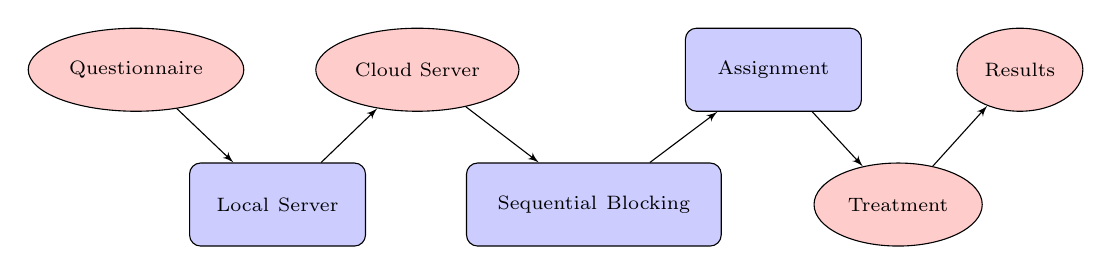
\begin{tikzpicture}
    \node [cloud]  (questionnaire) {\scriptsize{Questionnaire}};
    \node [block2, below right=0.8cm and -0.3cm of questionnaire] (local) {\scriptsize{Local Server}};
    \node [cloud, right= 0.9cm of questionnaire] (cloud) {\scriptsize{Cloud Server}};
    \node [block3, below right=0.8cm and -0.3cm of cloud] (sequential) {\scriptsize{Sequential Blocking}};
    \node [block2, right= 2.1cm of cloud] (assignment) {\scriptsize{Assignment}};
    \node [cloud, below right=0.8cm and -0.3cm of assignment] (treatment) {\scriptsize{Treatment}};
    \node [cloud, right= 1.2cm of assignment] (results) {\scriptsize{Results}};
    \path [line] (questionnaire) -- (local);
    \path [line] (local) -- (cloud);
    \path [line] (cloud) -- (sequential);
    \path [line] (sequential) -- (assignment);
    \path [line] (assignment) -- (treatment);
    \path [line] (treatment) -- (results);
\end{tikzpicture}
\caption{Online Survey Experiment Workflow} \label{online-workflow}
\end{figure}

The user uploads the complete survey questionnaire, i.e.~questions that
collect demographic information and questions that apply treatment, as a
\texttt{.csv} file into R. The \texttt{shiny} function within the R
package creates a web survey structure by employing the user's R
environment as the local `host server'. This means that the survey is
not accessible on the web yet -- it is located on the user's local
computer environment. To make the survey public, the user hosts this
website on a cloud server (e.g.~Amazon Web Services, Blue Ocean). The
created cloud-based public website is used directly to recruit
participants. The website sequentially blocks each incoming participant
based on her covariate information and covariate information from all
previous participants. This is done through constant interaction with
the R code provided by \texttt{BlockExperiments}, which is integral to
the website build. Based on the sequential blocking, the incoming
participant is assigned to a treatment group and then receives the
appropriate treatment. Her responses are then saved on the server. This
process is repeated for all incoming participants.

To recruit participants, the cloud-based website can easily be linked to
online market platforms, such as MTurk. MTurk is a service where
researchers can host tasks to be completed by anonymous participants.
Participants receive financial compensation for their work and Amazon
collects a commission. MTurk samples have been shown to be internally
valid in survey experiments \citep{berinsky_evaluating_2012}. The use of
MTurk in political science experiments has increased dramatically over
the past decade and is now common practice
\citep{hauser_attentive_2016}.

For online survey experiments, \texttt{BlockExperiments} thus creates
its own web-based survey. A theoretic alternative to this approach is to
use online survey design platforms, such as Qualtrics. Since Qualtrics
is very popular, it would appear fruitful to have
\texttt{BlockExperiments} load questions directly into Qualtrics,
instead of hosting the questions on a remote website via \texttt{shiny}.
However, this idea appears not computationally feasible. There have been
attempts to combine R code work with Qualtrics:

\citet{hainmueller_2014_causal} show how conjoint analysis enables
researchers to estimate the causal effects of multiple treatment
components and assess several causal hypotheses simultaneously. To do
so, they develop a computer program that creates conjoint question
design templates. The program exports the templates as a \texttt{.php}
file, which is then uploaded to a web server, which can then in turn be
loaded into Qualtrics via the Qualtrics functions Web Service and
Embedded Data. This pipes the file into the Qualtrics question design
environment. While this facilitates conjoint survey questionnaire
design, it does not affect Qualtrics's randomization engine but `only'
loads question categories. \citet{barari_2017_package} develop the R
package \texttt{cjoint}, which is designed to calculate Average Marginal
Component Effects of conjoint survey data. It has a function called
\texttt{makeDesign} which creates the conjoint survey design from output
created by \citet{hainmueller_2014_causal}'s Conjoint Survey Design Tool
and also contains two functions that pull the final \texttt{.csv} file
from Qualtrics directly into R. This tool then addresses the data
analysis after the survey has run, but not Qualtrics's randomization
engine. Similarly, the R package \texttt{QualtricsTools}
\citep{testa_2017_qualtricstools} provides functions to analyze
Qualtrics survey data by automatically processing the data into reports
breaking down the responses to each question. A similar function is
offered by the R package \texttt{qualtRics} \citep{ginn_2018_package},
which pulls survey data from Qualtrics to analyze directly in R through
the Qualtrics APIs.

None of these tools, then, concern the `injection' of R code into the
Qualtrics randomization engine. \citet{boas_fielding_2013} recommend
using the R web tool \texttt{shiny} to achieve this as it is
purposefully built to easily harnesses all the statistical power from R.
It thus seems a much more feasible vehicle for my project.

\subsection{Data}\label{seq-data}

I demonstrate the improvements produced by my sequential blocking method
by comparing balances in data with ordinal covariates from several data
sources: Simulations, others' external data, and my own original survey
data. In each source of data, I focus on the two ordinal variables that
are most common and most important in political science: Income and
education.

\subsubsection{Simulated Data}\label{seq-data-simulated}

I simulate an experiment with common demographic covariates, such as
age, race, gender, income, education, and party ID. The sample size is
1,000 participants, which is a common sample size for political science
survey experiments. The experiment features 5 treatment groups, which
results in around 200 participants per treatment group. Compared to
prominent survey experiments such as \citet{chong_framing_2007}, who
have fewer than 900 participants for 17 treatment groups, this is a
conservative setup. The outcome variable is irrelevant, since we are
only interested in balance here. I employ two separate randomization
methods: Complete randomization, and my sequential blocking method. Each
method is simulated 1,000 times. This means I simulate 1,000 runs of
this experiment with complete randomization, and another 1,000 runs of
this experiment with my sequential blocking method. The comparison of
the distribution of the blocked \(d^2\) \(p\)-values and the complete
randomization balance demonstrates balance improvements produced by my
method.

\subsubsection{External Data}\label{seq-data-external}

I also use data from external experimental survey studies and
sequentially block the participants in these data for ordinal
covariates. To create a sequential nature, I assume that the order of
the observations in the replication data file represents their entry
order into a sequential experiment. One example for such data is
\citet{tomz_2013_public}, who explore whether American participants are
more likely to support pre-emptive military strikes on non-democracies
versus democracies. The authors present participants with different
country profiles and ask participants whether they would support
pre-emptive American military strikes against the hypothetical country.
They randomly assign various characteristics of these profiles,
including (1) whether the country is a democracy, (2) whether the
country has a military alliance with the United States, and (3) whether
the country has a high level of trade with the United States. As before,
however, the outcome variable is irrelevant, since we are only
interested in balance. I plan to use up to four suitable similar
experimental survey data here, including
\citet{hainmueller_2014_causal}'s conjoint experiment data. If possible,
I also plan to obtain the data from \citet{chong_framing_2007} (which is
currently not publicly available).

With published peer-reviewed data, it is to be expected that the
experiments are overall well-balanced, i.e. \(p \approx 0.9\)
\citep{moore_blocking_2013}. Nonetheless, I expect a comparison of the
distribution of the blocked \(d^2\) \(p\)-values and the balance in the
original experiment to improve balance. \citet{moore_blocking_2013} show
that sequential blocking can indeed make overall balance in
well-balanced experiments nearly perfect.

\subsubsection{Original Data}\label{seq-data-original}

For the final application, I employ original survey data. I design a
questionnaire to assess the effect of moral frames on public opinion in
a survey experiment. This questionnaire is fielded online on MTurk for a
random sample of U.S. adults and face-to-face for undergraduate students
at American University. In each experiment, I use my sequential blocking
method on ordinal covariates to assign participants to treatment groups.
While I analyze the substantive results in depth in
\protect\hyperlink{paper-iii-moral-arguments-as-a-source-of-frame-strength}{paper
III}, they are irrelevant here, as we are only interested in balance. I
then use the collected covariate information and re-assign participants
to treatment groups with complete randomization. As before, the
comparison of the distributions of the blocked \(d^2\) \(p\)-values and
the complete randomization balance demonstrates balance improvements
produced by my method.

\clearpage

\hypertarget{paper-ii-measuring-mode-effects-for-ordinal-survey-responses-in-online-and-face-to-face-survey-experiments}{\section{Paper
II: Measuring Mode Effects for Ordinal Survey Responses in Online and
Face-to-Face Survey
Experiments}\label{paper-ii-measuring-mode-effects-for-ordinal-survey-responses-in-online-and-face-to-face-survey-experiments}}

\addtocontents{toc}{\protect\addvspace{8pt}}

\subsection{Introduction}\label{mode-intro}

Survey methodology is continuously undergoing changes. One prominent
area of such change is survey mode. Survey mode refers to the manner in
which survey responses are collected. The most common survey modes are
face-to-face interviews, mailed letters, telephone calls, and online
questionnaires. Up until the 1970s, mail and face-to-face surveys were
the main modes of data collection \citep{lyberg_1991_data}. Because of
the low costs of telephone calls and based on the ever-increasing phone
network coverage across the US, survey researchers then gradually
shifted to telephone calls, which soon replaced face-to-face interviews
as the most widely used survey mode, particularly through the use of
random-digit dialing \citep{dillman_2000_mail}. It is much cheaper to
call potential respondents from your desk than to travel to each
respondent's place of residence for an interview. In the 1990s, the
emergence of the internet challenged the supremacy of the telephone to
conduct surveys \citep{brick_2011_future}. It is much cheaper still to
create one digital questionnaire and provide it online than to call and
talk to potential respondents for hours.

Changes in mode choice can be problematic. Each mode can influence the
way participants think about and respond to survey questions, which in
turn hurts comparability of surveys across modes. This influence is
called `mode effects'. Mode effects form a key part of the Total Survey
Error (TSE) framework. The TSE consists of five primary sources of error
in survey research: Sampling error, coverage error, nonresponse error,
measurement error, and post-survey error \citep{weisberg_2005_total}. It
comprises all potential errors that can occur whilst conducting a sample
survey and using model-based statistical means to describe a population
\citep{biemer_2010_overview}. Survey mode choice can `activate' each and
all of these sources of error
\citep{groves_2010_total, weisberg_2005_total, ansolabehere_2014_does, atkeson_2014_nonresponse, ye_2011_more, yeager_2011_comparing, bowyer_2017_mode}.

While research is able to pinpoint certain parts of surveys where
respondents' reactions are and are not affected by mode, the literature
offers little help in identifying whether systematic mode effects exist
that affect the distributions of responses and the survey instrument as
a whole. For instance, is there a measurement error in the form of a
critical distributional difference in aggregate survey responses? If
there is such a distributional measurement error, what potential do such
a measurement and its related findings have? Can it affect how we
interpret question responses given on each respective mode? Do such
systematic differences occur, and if so, when do they occur, and do they
matter?

In an attempt to address this question, \citet{homola_2016_measure}
develop an entropy measurement \citep{shannon_1948_mathematical} for
discrete survey measures. Entropy roughly translates to `information'
and is most often used in information theory to carry levels of
information in a message. Entropy represents a measure of the average
amount of information that is required to describe the distribution of a
variable of interest \citep{cover_1991_elements}. They find that entropy
catches differences in mode effects that traditional statistical
measurements that assume continuous data, e.g.~the standard deviation,
miss: Mode effects do not show in measures of centrality, but instead
are shown by greater variability. \citet{homola_2016_measure} show that
entropy is a good measure of variability for discrete survey measures as
it reveals differences in how respondents react to identical questions
presented in two differing modes.

Entropy thus shows great potential to uncover distributional differences
in responses between survey modes. In its application to political
science data, however, Homola et al.'s measure falls short on the aspect
of ordinality. In political science, two of the most important
predictors of political behavior are ordinal survey measures: Education
and income. Income, for instance, is a strong predictor for political
behavior such as turnout, representation, or donations
\citep{dawood_campaign_2015, fiorina_disconnect_2009, leighley_who_2014}.
\citet{homola_2016_measure} do not account for ordinality in their model
and there is currently no way to measure entropy for these important
ordinal survey measures. I fill this gap by developing such a
measurement. I apply it to two modes: Online and face-to-face.
Substantively, I employ this measure in external data from political
science experiments published in peer-reviewed journal articles and
original data in the form of an online and face-to-face survey
experiment on the importance of moral arguments in political framing.

The following sections describe the TSE framework in more detail and put
it in connection with research on mode effects, showcase Homola et al.'s
entropy measurement, develop a measurement for ordinal entropy, and
provide a brief overview of the data sources I use to employ this
measurement.

\subsection{Theory}\label{mode-theory}

\subsubsection{Total Survey Error (TSE)}\label{mode-theory-tse}

As mentioned above, the TSE is an overarching framework that gives a
complete account of the potential errors that can result from conducting
a sample survey and using model-based statistical means to describe a
population \citep{biemer_2010_overview}. It ``is based on analyzing the
several different sources of error in surveys and considering how to
minimize them in the context of such practical constraints as available
money'' \citep[p.~16]{weisberg_2005_total}. `Error' here refers to the
difference between the values the researcher obtains and the `true
value' she should obtain.

There are five primary sources of error in the TSE: Sampling error,
coverage error, nonresponse error, measurement error, and post-survey
error
\citep{groves_2010_total, groves_survey_2009, weisberg_2005_total}.
Survey mode can affect each and all of these sources. They are
diagrammed in Figure \ref{tse-model} which shows the order of concern
that each potential source of error appears in the survey data
collection process. The arrows in the figure represent this sequential
nature, rather than causal paths. Figure \ref{survey-life-cycle} locates
the five potential sources of error more precisely within the survey
life cycle.

\vspace{0.4cm}

\begin{figure}[H]
\centering
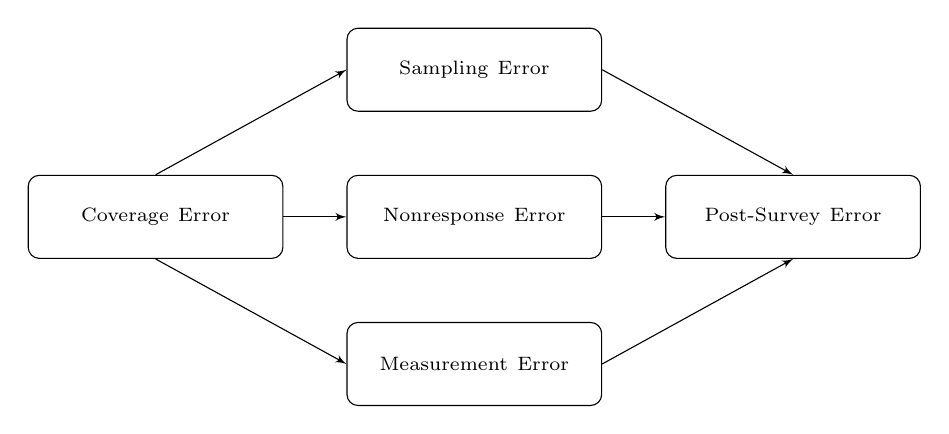
\begin{tikzpicture}
    \node [block4]  (nonresponse) {\scriptsize{Nonresponse Error}};
    \node [block4, left= 0.8cm of nonresponse] (coverage) {\scriptsize{Coverage Error}};     
    \node [block4, right= 0.8cm of nonresponse] (postsurvey) {\scriptsize{Post-Survey Error}};
    \node [block4, below= 0.8cm of nonresponse] (measurement) {\scriptsize{Measurement Error}};
    \node [block4, above= 0.8cm of nonresponse] (sampling) {\scriptsize{Sampling Error}};
    \path [line] (coverage.north) -- (sampling.west);
    \path [line] (coverage) -- (nonresponse);
    \path [line] (coverage.south) -- (measurement.west);
    \path [line] (sampling.east) -- (postsurvey.north);
    \path [line] (nonresponse) -- (postsurvey);
    \path [line] (measurement.east) -- (postsurvey.south);
\end{tikzpicture}
\caption{Model of Total Survey Error (from Homola et al. 2016)} \label{tse-model}
\end{figure}

\begin{figure}[H]
\centering
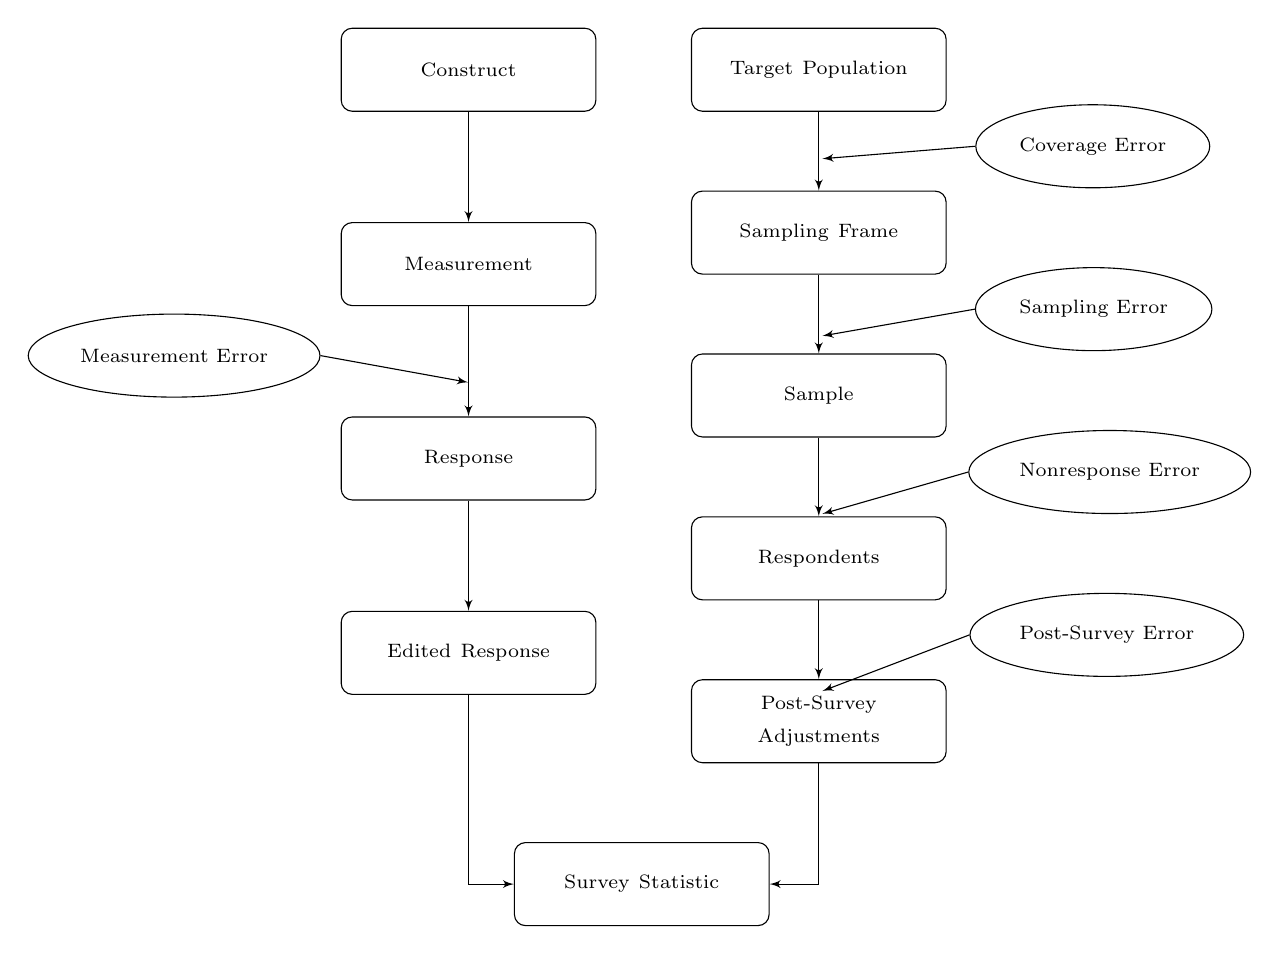
\begin{tikzpicture}
    \node [block4]  (construct) {\scriptsize{Construct}};
    \node [block4, below= 1.4cm of construct] (measurement) {\scriptsize{Measurement}};
    \node [cloud2, below left=0.25cm and 0.8cm of measurement] (measurement_error) {\scriptsize{Measurement Error}};
    \node [block4, below= 1.4cm of measurement] (response) {\scriptsize{Response}};     
    \node [block4, below= 1.4cm of response] (edited) {\scriptsize{Edited Response}};  
    \node [block4, right= 1.2cm of construct] (target) {\scriptsize{Target Population}};     
    \node [cloud2, below right=0.06cm and 0.8cm of target] (coverage_error) {\scriptsize{Coverage Error}};
    \node [block4, below= 1cm of target] (sampling) {\scriptsize{Sampling Frame}};     
    \node [cloud2, below right=0.06cm and 0.8cm of sampling] (sampling_error) {\scriptsize{Sampling Error}};
    \node [block4, below= 1cm of sampling] (sample) {\scriptsize{Sample}};     
    \node [cloud2, below right=0.06cm and 0.8cm of sample] (nonresponse_error) {\scriptsize{Nonresponse Error}};
    \node [block4, below= 1cm of sample] (respondents) {\scriptsize{Respondents}};     
    \node [cloud2, below right=0.06cm and 0.8cm of respondents] (postsurvey_error) {\scriptsize{Post-Survey Error}};
    \node [block4, below= 1cm of respondents] (postsurvey) {\scriptsize{Post-Survey Adjustments}};     
    \node [block4, below left= 1cm and -1cm of postsurvey] (statistic) {\scriptsize{Survey Statistic}};     
    \path [line] (construct) -- (measurement);
    \path [line] (measurement) -- (response);
  \path [line] (measurement_error.east) -- (-0.006cm,-3.97cm);
    \path [line] (response) -- (edited);
  \path [line] (edited.south) |- (statistic);
    \path [line] (target) -- (sampling);
  \path [line] (coverage_error.west) -- (4.495cm,-1.13cm);
    \path [line] (sampling) -- (sample);
  \path [line] (sampling_error.west) -- (4.495cm,-3.38cm);
    \path [line] (sample) -- (respondents);
  \path [line] (nonresponse_error.west) -- (4.495cm,-5.64cm);
    \path [line] (respondents) -- (postsurvey);
  \path [line] (postsurvey_error.west) -- (4.495cm,-7.89cm);
  \path [line] (postsurvey.south) |- (statistic);
\end{tikzpicture}
\caption{Survey Life Cycle (adapted from Groves et al. 2009)} \label{survey-life-cycle}
\end{figure}

As shown in Figure \ref{survey-life-cycle}, all sources add up to form
one resulting total survey error, or TSE. I now address each of the five
sources and their explicit connection to survey mode in turn.

\subsubsection{Five Types of Survey Error in Connection with Survey
Mode}\label{mode-theory-types}

\paragraph{Coverage Error}\label{mode-theory-types-coverage}

Coverage error applies to the nonobservational gap between the target
population and the sampling frame, i.e.~the actual set of units from
which the sample is taken \citep{groves_survey_2009}. This means we
choose a sample intended to represent the target population from a
sampling frame that does not actually cover that target population. In
statistical terms, coverage error is the mathematical difference between
a statistic calculated for the population that is studied and the same
statistic calculated for the target population
\citep{weisberg_2005_total}.

In early survey research days, potential survey respondents could only
be contacted through mailed letters. Since everyone in the target
population, i.e.~the U.S. population, had a mailing address, the
sampling frame of mailing addresses was identical to the target
population, both for questionnaires sent directly through the mail and
for mailed requests for face-to-face interviews. The invention of the
telephone provided a cheaper, faster alternative. Until around 35 years
ago, however, telephone landline access did not cover the entire U.S.
population, so any samples drawn from a list of landline phone numbers
did not cover the entire adult U.S. population. In such a case, there
are population units that fall outside of the sampling frame because of
the chosen vehicle of communication, i.e.~the survey mode. People who
did not have telephones could not be contacted and were thus not part of
the sampling frame. Since people who did not yet have telephones were
likely to differ systematically from people who did have them, this lead
to biased estimates of the variables of interest. In other words, bias
occurred because non-covered units were omitted from the sample because
of the choice of survey mode.

In more current times, this issue arises for people who no longer have a
landline but instead rely exclusively on their cell phone. If the chosen
vehicle of communication is landline telephone numbers, these people
will be excluded from the sample. In 2008, 17.5 percent of U.S.
households had only wireless telephone access, with landline coverage
having decreased to 80 percent \citep{blumberg_2008_recent}, with this
trend likely to have continued in the years to follow. Similarly,
coverage error can be substantial in online surveys intended to
represent the U.S. population, as 11 percent of U.S. adults currently do
not have access to the internet \citep{pew_2018_internet}. This number
continues to shrink, however, with the continuous spread of high-speed
internet access in rural areas.

\paragraph{Sampling Error}\label{mode-theory-types-sampling}

Researchers can only very rarely ask an entire population but instead
have to rely on samples. As a result, not all people in the sampling
frame, i.e.~the entire population, are part of the eventual sample. This
nonobservational gap between the sampling frame and the sample is called
sampling error \citep{groves_survey_2009}. Sampling error is thus very
much by definition part of survey data collection. It is often
colloquially known as the `margin of error', i.e.~the difference in
estimates between repeated samples.

Sampling error primarily arises in the form of sampling bias. Sampling
bias occurs when some units of the sampling frame are systematically
excluded from the sample. This can be avoided by probability sampling,
i.e.~randomly selecting units of the sampling frame to be included in
the sample. It is essential here that everyone in the larger population
has a known probability of being chosen for the random sample. This is
not the case with non-probability sampling, also known as convenience
sampling, where researchers collect responses of everybody who
conveniently `stops by' to answer questions. In non-probability
sampling, sampling bias can be systematic. While this can affect all
survey modes, it is a particular problem for online surveys, where
participants volunteer to answer questions, often in return for
financial compensation \citep{ansolabehere_2014_does}. One such example
is MTurk (see section \ref{seq-computational-r} of Paper I for a brief
outline of MTurk). These volunteers can differ systematically from
participants who are randomly selected and can look very different in
terms of their covariates than the rest of the population
\citep{dillman_2014_internet, couper_2000_surveys, hays_2015_internet, alvarez_2003_subject}.

\paragraph{Measurement Error}\label{mode-theory-types-measurement}

Measurement error is ``the error that occurs when the measure obtained
is not an accurate measure of what was to be measured''
\citep[p.~18]{weisberg_2005_total}. In other words, the questions that
researchers choose to measure something do not actually measure that
thing. Measurement error is the observational gap between the ideal
measurement and the response obtained \citep{groves_survey_2009}. There
are two primary levels of measurement error: Respondent-induced
measurement error and interviewer-induced measurement error.
Respondent-induced measurement error occurs when respondents do not give
the answers they `should' give. The most common respondent-induced
measurement errors are non-differentiation and speeding.

Non-differentiation involves participants who give answers that simply
enable them to finish the survey as quickly as possible. For online
surveys, this means that the impersonal screen interface could lead
people to simply select the same answer for every question, something
they could not do with a human interviewer. \citet{chang_2010_comparing}
utilize a true random assignment to either self-administered computer
surveys or interviewer-enabled RDD phone interviews. They find that
online participants provide fewer straightlining answers than RDD
participants. Contradicting these findings,
\citet{heerwegh_2008_face-to-face} uncover more `straightlining' in
web-based surveys than face-to-face. Similarly,
\citet{fricker_2005_experimental} find evidence for more
`straigthlining' in web-based experiments than through the phone.
Speeding concerns responses that were given `too fast', given the number
and depth of survey questions. Most research shows that online surveys
display more speeding than other modes
\citep{chang_2010_comparing, miller_2000_phone, heerwegh_2008_face-to-face, greszki_2015_exploring}.
It is important to note, however, that speeding might not necessarily be
bad for response quality. It could simply be that a visual mode of
seeing the questions enables people to answer with the same quality,
just more quickly than merely hearing the questions. Speeding research
has yet to develop a method to distinguish these aspects.

Interviewer-induced measurement error occurs when the interviewer
influences how respondents answer the questions. The most common
interviewer-induced measurement error is social desirability bias. The
social desirability hypothesis proposes that in the presence of an
interviewer, some participants may be reluctant to admit embarrassing
attributes about themselves or may be motivated to exaggerate the extent
to which they possess admirable attributes
\citep{chang_2010_comparing, rogers_2001_using}. This body of research
is consistent with the notion that self-administration by computer
elicits more honesty \citep{kreuter_2008_social}. In other words, people
are more honest when they answer sensitive questions on a screen than
when they talk to another human being directly (be that face-to-face or
on the phone). Other potential sources for interviewer-induced
measurement error include gender, race, and age
\citep{huddy_1997_effect, rooney_2005_effects, tourangeau_2007_sensitive, warnecke_1997_improving, yan_2008_fast}.

\paragraph{Nonresponse Error}\label{mode-theory-types-nonresponse}

Nonresponse error applies to the nonobservational gap between the sample
and the respondent pool \citep{groves_survey_2009}. Nonresponse error
can occur on two levels, namely the unit and the item. Unit nonresponse
error arises when a respondent who was supposed the answer the survey
does not do so. Item nonresponse error happens when a respondent does
not answer all questions or provides `Don't Know' as an answer to one or
several questions. It is very common for response rates to be very low,
often in the area of 10 percent \citep{groves_survey_2009}. This need
not necessarily be worrisome, as long as these 10 percent look like the
other 90 percent in terms of their covariates. It is only when
differences between respondents and nonrespondents are systematic that
nonresponse error comes into play. A high nonresponse rate does not
equal the existence of bias, the same way a low nonresponse rate does
not protect from bias. However, it is generally thought that a low
nonresponse rate is preferred because it reduces the risk of nonresponse
bias while not offering complete protection \citep{weisberg_2005_total}.

An abundance of studies on nonresponse in connection with survey mode
exist. \citet{atkeson_2014_nonresponse} find significant differences of
nonresponse between telephone and online surveys, yet also show evidence
that both modes represent the underlying population well. Somewhat
similarly, \citet{nagelhout_2010_interviewing} uncover differences
between a web and telephone sample but maintain that these differences
were small and not consistently favorable to either survey mode. On the
contrary, \citet{couper_2001_promises} finds significant differences in
nonresponse rates across modes. He concludes that nonresponse is a
crucial concern for online surveys, especially when compared to the
alternative method of mail. On the other hand,
\citet{chang_2010_comparing} identify lower nonresponse rates in
computer surveys when compared to those administered by phone. They thus
tentatively suggest a potential advantage of the online mode over
telephone administration. Yet contrary again,
\citet{west_2013_interviewer} emphasize interviewers' ability to
influence hesitant participants on the phone and face-to-face, which is
not possible online. \citet{dillman_2005_survey} in turn point out that
nonresponse in online surveys can be overcome by software setup that
obliges participants to answer all questions. These severely differing
findings indicate that is far from clear whether there is a systematic
difference in the levels of nonresponse and whether such a difference
results in differing levels of data quality
\citep{groves_2010_total, mcnabb_2013_nonsampling, millar_2012_mail, aapor_2013_report}.

\paragraph{Post-Survey Error}\label{mode-theory-types-post}

Once data collection is completed, researchers often apply various
statistical methods to adjust and improve the obtained results. These
undertakings are best described as post-survey ``efforts to improve the
sample estimate in the face of coverage, sampling, and nonresponse
errors'' \citep[p.~59]{groves_survey_2009}. Any error that arises in
this stage, when the survey data is processed and analyzed, is called
post-survey error. Post-Survey error concerns everything that happens to
survey data after collection is finished and includes data cleaning,
recoding, weighting, and modeling, among many others
\citep{weisberg_2005_total}. Whilst applicable to all survey modes,
weighting and modeling to create representative survey results is
heavily used and widely spread particularly in online surveys
\citep{atkeson_2014_nonresponse}. Any of these procedures can introduce
error to the survey analysis process and thus bias the estimate
\citep{mcnabb_2013_nonsampling}.

\subsubsection{Entropy}\label{mode-theory-entropy}

\paragraph{Entropy for Discrete Survey
Responses}\label{mode-theory-entropy-discrete}

Research on mode effects within the TSE thus does not reveal much about
systematic, distributional differences that might be caused by mode
choice. In particular, ``despite the widespread use of online panels,
there is still a great deal that is not known with confidence''
\citep[p.~54]{aapor_2010_opt-in}. In an attempt to address this issue,
\citet{homola_2016_measure} develop an entropy measurement
\citep{shannon_1948_mathematical} for discrete survey measures. They
argue that traditional statistical measurements, such as the variance
(Var\((X) = \frac{1}{n-1} \sum (X_i - \overline{X})^2\)) and the median
average deviation
(MAD\((X) =\)median\((\vert X_i -\)median\((X)\vert\)), appear unsuited
to the task of assessing this aspect as they assume interval measured
data. In particular, \(\overline{X}\) and median\((X)\) are said to not
represent correct measures of centrality
\citep{homola_2016_measure, wang_2008_probability, hu_2010_information}.
Entropy, on the other hand, is a measure of variability in discrete
survey responses \citep{shannon_1948_mathematical}.

Entropy roughly translates to `information' and is most often used in
information theory to carry levels of information in a message. It
represents a measure of the average amount of information that is
required to describe the distribution of a variable of interest
\citep{cover_1991_elements}. Mathematically, Homola et al.'s entropy
measure for a given response is formed by empirically counting the
observations in each survey mode and subsequently normalizing them into
probabilities. This measure, \(H\), is calculated by

\[H(X) = \sum\limits_{i=1}^{n} p(x_i) \text{log}_2 (\frac{1}{p(x_i)})\]

where \(p(x_i) = Pr(X=x_i)\) is the probability of the \(i^{\text{th}}\)
outcome of \(X\). The entropy of the variable \(X\) is thus the product
of the probability of outcome \(x_i\) and the log of the inverse of the
probability of \(x_i\), summed over all possible outcomes \(x_i\) of
\(X\).

Based on \citet{shannon_1948_mathematical}, \citet{homola_2016_measure}
argue that entropy is the only function that satisfies three critical
properties: (1) \(H\) is continuous in the discrete measure
\({p_1,p_2,...,P_n}\), (2) \(H\) is at its maximum and is monotonically
increasing with \(n\) if the \(p_i\) are uniformly distributed, and (3)
The first \(H\) equals the weighted sum of consecutive \(H\) values,
\(H(p_1,p_2,p_3) = H(p_1, 1-p_1) + (1 - p_1) H (p_2, p_3)\).
Additionally, entropy does not make assumptions about the probability
distribution of the variability of uncertainty.

Applying their measure to the 2012 ANES, which used identical questions
that were asked face-to-face and online, \citet{homola_2016_measure}
find that entropy catches differences in mode effects that traditional
statistical measurements that assume continuous data, e.g.~the standard
deviation, miss: Mode effects do not show in measures of centrality, but
instead are shown by greater variability. They show that entropy reveals
differences in how respondents react to identical questions presented in
two differing modes. Their measure does not, however, account for
ordinal variables, which are crucial in political science research.

\paragraph{Entropy for Ordinal Survey
Responses}\label{mode-theory-entropy-ordinal}

Why do we need an entropy measurement that accounts for ordinal
variables? \citet{homola_2016_measure} demonstrate that entropy reveals
a measurement error in the form of a critical distributional difference
in aggregate survey responses that traditional statistical measurements
miss. Traditional statistical measurements also suppose ordinal data
with roughly equally spaced distances between levels. Popular political
science surveys, such as the ANES and the majority of survey
experiments, however, contain ordinal data which are not equally spaced.
\citet{johns_2005_size}, for example, points out that response scales
that measure support or opposition often show significant differences in
terms of spacing. On a 5-point Likert scale, the neighboring points 2
(``Somewhat oppose'') and 3 (``Neither favor or oppose'') are much
closer together than the neighboring points 1 (``Strongly oppose'') and
2. Ordinality is a crucial feature of these variables. Treating ordinal
variables as numerical results in the loss of this information of two
crucial variables that predict political behavior. The lack of
ordinality in an entropy measurement thus excludes two of the most
important predictors of political behavior from survey mode effects
analysis.

To develop a measure of ordinal entropy, I combine the Wilcoxon Signed
Rank Test (WSRT) and Shannon's entropy measure to obtain a comparative
measure of two ordinal vectors. The WSRT considers ordinal data as
`ranks'. By definition, ranks are not affected by outliers, since no
outlying value is more than one unit away from the next value. The WSRT
removes information about the distributional shape of the data. It is a
statistical hypothesis test to compare two related samples to assess
whether their population mean ranks differ, i.e.~a paired difference
test. It is used to determine whether two dependent samples were
selected from populations that show the same distribution.

The WSRT follows several concrete steps. Let the first sample be denoted
by units \(x_{11}, x_{12}, ..., x_{1n}\) and the second sample by units
\(x_{21}, x_{22}, ..., x_{2n}\). We pair the units across samples,
\((x_{11}, x_{21}), (x_{12}, x_{22}), ..., (x_{1n}, x_{2n})\), and
define the paired differences,
\(d_1 = x_{11} - x_{21}, d_2 = x_{12} - x_{22}, ..., d_n = x_{1n} - x_{2n}\).
We obtain the absolute value and sign of the paired differences and
subsequently rank them, with values equaling zero being discarded. Let
us call these values \(R_1, R_2, ..., R_{n'}\), where the new \(n' < n\)
because of the discards that were carried out. We then calculate:

\[T^+ = \Bigg\vert \sum\limits_{i=1}^{n'} \text{sign}(d_i) \times R_i \Bigg\vert = \Bigg\vert \sum\limits_{i=1}^{n'} \text{signed rank of } d_i \Bigg\vert\]

The null hypothesis of the WSRT is \(H_0\): median\((\delta) = 0\), with
the alternative hypothesis being \(H_A\): median\((\delta) \neq 0\). The
new ordinal entropy measure I propose is simply the combination of the
WSRT and Homola et al.'s entropy measure:

\[T^+ = \Bigg\vert \sum\limits_{i=1}^{n'} \text{signed rank of } d_i \times \text{log}_2 (\frac{1}{p(d_i)}) \Bigg\vert\]

In the original WSRT, the \(\text{signed rank of } d_i\) are defined as
the signed ranks of all paired absolute differences \(d_i\). In our
modified case, the \(\text{signed rank of } d_i\) are simply the signed
ranks of the paired absolute differences between the two ordinal vectors
of the two mode samples.

\subsection{Data}\label{mode-data}

I apply my new method of ordinal entropy to external and original data
in the online and face-to-face modes. For both purposes, I intend to
conduct parallel studies with identical questions in the same period of
time. I calculate ordinal entropy measurements for each survey mode.
This reveals systematic, distributional differences that might be caused
by mode choice. I then contrast these measures with the most common
measure of the TSE for measures with validated baselines and the total
survey measurement variation approach for questions on opinions and and
attitudes. The most common measure of the TSE is the mean squared error,
i.e.~the squared average deviation of a survey estimate from the true
value of the parameter being estimated. A large mean squared error
indicates ``that one or more sources of error are adversely affecting
the accuracy of the estimate'' \citep[p.~826]{biemer_2010_total}. For
measures without validated baselines, i.e.~questions regarding opinions
and attitudes that lack previous survey exposure, I estimate the extent
to which the surveys produce diverging measures of each concept in the
respective survey modes \citep{smith_2011_refining}.

\subsubsection{External Data}\label{mode-data-external}

External data sets with identical questionnaires face-to-face and online
modes are provided by the 2012 ANES, as used by
\citet{homola_2016_measure}, the 2016 ANES, and several Pew surveys. The
Pew Research Center in particular has excelled in gradually shifting its
modes. This provides an ideal testing ground to prove the validity of
the ordinal entropy measure. I demonstrate that ordinal entropy matters
when switching survey modes, as the new measure reveals discrepancies
that cannot be detected with traditional statistical measurements (see
section \ref{mode-theory-entropy-ordinal}).

\subsubsection{Original Data}\label{mode-data-original}

In addition to external data, I use original data to demonstrate ordinal
entropy discrepancies and why they are significant. For this purpose, I
field a survey experiment on the power of moral arguments online on
MTurk and face-to-face for undergraduate students at American
University. The details of this experiment can be found in
\protect\hyperlink{paper-iii-moral-arguments-as-a-source-of-frame-strength}{paper
III} below.

\clearpage

\hypertarget{paper-iii-moral-arguments-as-a-source-of-frame-strength}{\section{Paper
III: Moral Arguments as a Source of Frame
Strength}\label{paper-iii-moral-arguments-as-a-source-of-frame-strength}}

\addtocontents{toc}{\protect\addvspace{8pt}}

\subsection{Introduction}\label{framing-intro}

Barack Obama presented the first outline of the Affordable Care Act in
the summer of 2009. The content of the reform was put online for
everyone to see, but since the administration was still working on
details, it refrained from actively communicating it. Published press
releases simply stated that the ACA would expand coverage and lower
health care costs for everyone. This hesitancy turned out to be a big
mistake. At the end of July, support for the ACA hovered around 43
percent. Then Sarah Palin, John McCain's choice for running mate in
2008, posted the following statement on Facebook on August
7\textsuperscript{th}: ``The America I know and love is not one in which
my parents or my baby with Down Syndrome will have to stand in front of
Obama's `death panel' so his bureaucrats can decide, based on a
subjective judgment of their `level of productivity in society',''
\citep{palin_statement_2009}. Palin implied that federal government
workers would be able to refuse treatment to any patients and thus
`decide their fate'. Over the next two weeks, support for the ACA
dropped to 35 percent while opposition rose to 52 percent. Republican
lawmakers jumped at the opportunity and repeated the claim of `death
panels' whenever possible. The reform never recovered from this drop. In
December 2009, four months after the statement, support and opposition
were virtually identical to August. While the public was still uncertain
about the exact contents of the law, Palin had asserted that it would
include a Big Brother type panel that decided whether people would live
or die. This drowned out any efforts by the Obama administration to show
the law as a cost-reducing reform. Palin's frame of the ACA, in other
words, drastically influenced public opinion of the reform.

Framing is the practice of presenting an issue to affect the way people
see it
\citep{aaroe_investigating_2011, druckman_evaluating_2001, gross_framing_2008}.
We learn about healthcare reform through articles, reports, speeches,
commercials and social media. This mediated communication possesses
tremendous potential influence on our perception of political issues
\citep{iyengar_framing_1996, kam_risk_2010, tversky_framing_1981}.
Framing research has established that a variety of frames substantively
influence how people view and think about issues, such as the ACA
\citep{price_switching_1997, andsager_how_2000, callaghan_introduction_2005, entman_framing_1993, entman_projections_2004, gamson_media_1989, lahav_ideological_2012, pan_framing_1993, slothuus_political_2010, sniderman_structure_2004, vreese_effects_2004}.
But we do not know why these frames elicit these effects. A major
challenge for framing research thus ``concerns the identification of
factors that make a frame strong'' \citep[p.~116]{chong_framing_2007}.

I conduct a series of tests to examine whether moral arguments form a
part of what makes a frame strong. These tests include a meta-analysis,
three online polls, and a survey experiment that is fielded online and
face-to-face.

\subsection{Theory}\label{framing-theory}

\subsubsection{Framing}\label{framing-theory-framing}

Despite the mass of experimental framing research, we still have little
insight into what makes a frame strong. The larger persuasion literature
``is not as illuminating as one might suppose\ldots{} It is not yet
known what it is about the `strong arguments'\ldots{} that makes them
persuasive'' \citep{okeefe_2002_persuasion}. One research direction is
that frames are stronger overall when they cohere with an individual's
personal value system. \citet{feinberg_2012_moral} frame environmental
issues as a matter of `purity', a theme that supposedly correlates with
conservative ideology, and find this approach leads to increased
conservative support of environmental policies.
\citep[p.~280]{arceneaux_cognitive_2012} on the other hand finds that
``individuals are more likely to be persuaded by political arguments
that evoke cognitive biases''. Particularly, he asserts that messages
which highlight out-group threats resonate to a greater extent than
other, more coherent, arguments. In a study investigating the use of
scientific data, \citet{druckman_framing_2011} report that adding
factual information to messages about carbon nanotubes does nothing to
enhance their strength. Providing more scientific evidence seems to have
the opposite effect, making the messages weaker. Overall, ``it seems as
if frame strength increases with frames that highlight specific
emotions, invoke threat against one's own group interests, contain some
incivility, include multiple, frequently appearing, arguments, and/or
have been used in the past'' \citep[p.~22]{druckman_political_2018}. I
attempt to provide an avenue of clarification by testing whether moral
arguments are part of what makes frames strong.

\subsubsection{Moralization}\label{framing-theory-moralization}

Moralization literature conceptually defines moral arguments as (1)
near-universal standards of truth, (2) almost objective facts about the
world, and (3) independent of institutional authority
\citep{skitka_psychology_2010}. Moral arguments are said to engage a
distinctive mode of processing that invokes a whole range of emotions
and to be distinct from other forms of arguments
\citep{ryan_reconsidering_2014}. Scholars find that moral arguments are
ubiquitous in political issues because they are essential to how people
perceive and make sense of the world around them
\citep{frank_whats_2005, mooney_public_2001, tatalovich_moral_1994}.
\citet{ryan_reconsidering_2014} finds evidence that some people perceive
distinctly economic issues such as labor relations laws or social
security reform in moral ways. Other studies similarly assert that the
strength of attitudes meaningfully differs when they are held with moral
conviction
\citep{baron_protected_1997, bennis_costs_2010, ditto_motivated_2009, tetlock_correspondence_2003}.
It is also asserted that moral conviction represents an important force
that guides citizen behavior and development of public opinion
\citep{converse_nature_1964, skitka_moral_2005, skitka_moral_2011, smith_typologies_2002, tatalovich_moral_2011, zaller_nature_1992}.
It is widely argued that people rely to a disproportionate extent on
moral arguments to form their opinions and apply this moralization to
political issues
\citep{ryan_no_2014, ryan_reconsidering_2014, smith_typologies_2002}.
Moral arguments can achieve a much higher emotional connection with
people because they invoke people's values and feelings
\citep{skitka_moral_2005, skitka_moral_2011, haidt_moral_2003, tatalovich_moral_2011}.
These conceptual definitions are all encompassed in Moral Foundations
Theory (MFT), developed by \citet{haidt_2012_righteous} and presented in
Table \ref{framing-foundations} below.

\begin{table}[H]
\caption{Foundations of Moral Arguments}
\centering
\resizebox{\textwidth}{!}{
\begin{tabular}{>{\itshape}l ll >{\itshape}l l}
\bottomrule 
\midrule
\multicolumn{2}{c}{\textbf{Positive}} & & \multicolumn{2}{c}{\textbf{Negative}}\\
\cmidrule{1-2}
\cmidrule{4-5}
Care & Cherishing, protecting others & & Harm & Hurting others\\
Fairness & Rendering justice by shared rules & & Cheating & Flouting justice, shared rules\\
Loyalty & Standing with your group & & Betrayal & Opposing your group\\
Respect & Submitting to tradition, authority & & Subversion & Resisting tradition, authority\\
Sanctity & Repulsion at disgust & & Degradation & Enjoyment of disgust \\
\bottomrule
\multicolumn{5}{l}{\footnotesize{Based on Haidt (2012). Positive and negative foundations are conceptual opposites.}} \\
\end{tabular}}
\label{framing-foundations}
\end{table}

These aspects of moralization theory have not been applied to frame
strength in experimental research. An abundance of framing research has
shown that frames elicit significant changes in issue positioning
\citep{chong_counterframing_2013, chong_dynamic_2010, druckman_how_2013, druckman_limits_2001, druckman_source_2012, nelson_media_1997, slothuus_more_2008}.
\citet{brewer_values_2005}, for instance, find significant effects for
the frames `School vouchers create an unfair advantage' and `School
vouchers provide help for those who need it'.
\citet{druckman_source_2012} provide similar evidence for `The
Affordable Care Act gives more people equal access to health insurance'
and `The ACA increases government costs', while
\citet{druckman_how_2013} do so for `Oil drilling provides economic
benefits' and `Oil drilling endangers marine life'. While we know these
frames elicit changes, we do not know why they do so. We do not know why
these frames `work'. I propose a way to understand why some of these
frames work, which is based on moralization theory: The presence of
moral arguments.

Applying Moral Foundation Theory, both frames in
\citet{brewer_values_2005} could be categorized as containing moral
arguments, even though the authors do not explicitly do so. `School
vouchers create an unfair advantage' can be argued to contain the
negative moral foundation of \textit{Cheating}, while `School vouchers
provide help for those who need it' contains the positive moral
foundations of \textit{Care} and \textit{Fairness}. `The ACA gives more
people equal access to health insurance' \citep{druckman_source_2012}
also could be said to contain the positive moral foundations of
\textit{Care} and \textit{Fairness}, while `Oil drilling endangers
marine life' \citep{druckman_how_2013} contains the negative moral
foundation of \textit{Harm}.

It is important to note that `The ACA increases government costs'
\citep{druckman_source_2012} and `Oil drilling provides economic
benefits' \citep{druckman_how_2013} do not directly appeal to morality,
yet research has shown them to be strong. Of course, some people might
see increasing costs immediately as bad and thus morally detrimental for
the future of the country, but these frames do not make such an appeal
directly, on the surface. This distinguishes them from moral frames.

This might lead one to assert that moral arguments do not form a part of
frame strength -- after all, if a frame does not contain a direct moral
argument but is proven to be strong nonetheless, surely then frame
strength does not depend on the presence of moral arguments. This
hypothetical argument is flawed, however. For one, the search for the
source of frame strength is not the search for a universal `holy grail'
argument whose presence is a precondition for frame strength. There
probably are many aspects that can make a frame strong, with moral
arguments potentially being one of them, not the only one. Second, the
studies with these two amoral and two moral arguments do not distinguish
between the directions in which the moral and amoral frames act.

In the case of \citet{druckman_source_2012}, `The Affordable Care Act
gives more people equal access to health insurance' contains a positive,
i.e.~support-inducing, moral argument, while `The ACA increases
government costs' contains a negative, i.e.~opposition-inducing, amoral
argument. They act in opposite directions. A comparison of these frames
alone does not yield sufficient results as we would not be able to
identify the exact cause of the framing effect. Is `The Affordable Care
Act gives more people equal access to health insurance' strong because
it supports the issue or because it contains a moral argument?
Similarly, is `The ACA increases government costs' strong because it
opposes the issue or because it contains a amoral argument? This set-up
cannot answer these questions.

To establish whether moral arguments are part of what makes a frame
strong, we need a design that assesses the strength of frames with moral
and amoral arguments whilst accounting for both signs, opposing and
supporting, in both sets of frames. I provide such a design.

Overall, experimental framing research has shown that many frames have
significant framing effects. It is still unclear, however, what makes
these, or indeed any, frame strong \citep{druckman_political_2018}.
Moralization theory claims that moral arguments possess enormous power
shape human behavior and influence public opinion
\citep{haidt_moral_2003}. I combine these two sets of literature and
analyze whether moral arguments form a part of what makes frames strong.
I use a variety of data sources to investigate the following hypothesis:

\vspace{0.3cm}

\begin{adjustwidth*}{+1cm}{+1cm}
\textbf{H.} Moral arguments form a part of what makes political frames strong.
\end{adjustwidth*}

\subsection{Data}\label{framing-data}

First, I conduct a meta-analysis of all experimental framing surveys up
to the present day. The aim of this step is to obtain statistically
valid estimates of all the frames that have been shown to elicit
significant framing effects. Second, I field an online poll that asks
participant to assess how moral these researched frames are. Third, I
conduct a second online poll to obtain qualitative insights into what
people consider to be moral arguments. Fourth, I design and test moral
and amoral complementary frames to the ones used in previous research in
a third online poll, based on insights from the meta-analysis and the
two previous polls. Finally, I conduct the main online survey
experiment.

The insights gained from the second online poll are vital to the
designing of the frames. Possessing knowledge of the way people define
moral and pragmatic arguments is crucial to the development of frames
that accurately reflect these structures. To add a second layer of
insurance to protect against miss-designed frames, I also pre-test the
designed frames with participants who are not part of the main survey.
These participants are exposed to the designed frames and asked whether
they reflect the core ideas behind moral and pragmatic arguments. This
pre-test structure builds on work by \citet{slothuus_political_2010} and
\citet{chong_framing_2007}, following the mass communication and
persuasion literature \citep{okeefe_2002_persuasion}. The pre-test is
carried out on Amazon's online platform MTurk. Together with the
post-test included in the survey, the assessment of moral arguments and
a pre-test represent a thorough, robust, spread-out safety net to ensure
that the designed frames connect with participants, which in turn
ensures meaningful survey results.

\subsubsection{Meta-Analysis}\label{framing-data-meta}

A meta-analysis ``synthesizes the findings of many different scientific
studies of the same phenomenon'' through statistical analysis
\citep[p.~190]{groves_survey_2009}. The basic tenet behind meta-analyses
holds that there is a common truth behind all conceptually similar
scientific studies, but this truth has been measured with a certain
error within individual studies
\citep{schmidt_2015_methods, flores_2015_examining, greenland_2008_meta-analysis}.
A key benefit of this approach is the aggregation of information leading
to a higher statistical power and more robust point estimate than is
possible from the measure derived from any individual study
\citep{walker_2008_meta-analysis}. In performing a meta-analysis, an
investigator must make choices which can affect the results, including
deciding how to search for studies, selecting studies based on a set of
objective criteria, analyzing the data, and accounting for or choosing
not to account for publication bias
\citep{brockwell_2011_comparison, paterson_2001_meta-study, kuhberger_1998_influence, boulianne_2009_does}.

The first step in a meta-analysis is a comprehensive inventory of the
body of research. I use the large number of empirical framing studies I
analyzed over the years and supplement this by searching public
registries, such as \textit{Egap}. To account for publication bias, I
also include pertinent unpublished papers.

The second step is to develop criteria for inclusion. I only include
research with a focus on experimental framing. This means that studies
on related, but different, concepts such as priming or agenda-setting
and studies of a descriptive nature are excluded from the data.

The third step involves the calculation of effect sizes.There may be
areas of heterogeneity between the respective studies, such as differing
selection and treatment of subjects, or differences in the conception of
outcomes or policies \citep{roever_2017_bayesian}. This can be overcome
by using a Bayesian random effects model. In the Bayesian paradigm, the
unknown parameters involved in the model are considered random variables
\citep{gelman_2013_bayesian}. After eliciting a priori distributions,
these priors are combined with the empirical evidence (likelihood) to
obtain a joint posterior distribution, given the data we can observe.
Markov chain Monte Carlo (MCMC) methods can be used to obtain a sample
from the joint posterior distribution of the parameters. We use the
summaries of the marginal posterior distribution of the parameters of
interest (i.e.~in our case group means) to leverage inference \citep[all
from][]{gill_2014_bayesian}. The Bayesian approach accounts for the
uncertainty around the heterogeneity variance. Frequentist approaches
(e.g.~the \(t\) statistic), on the other hand, treat the estimate of the
variance as a fixed quantity, which results in variability
underestimation \citep{lau_1999_effects}.

\subsubsection{Online Poll \#1: The Moral Content of Frames Used in
Previous Studies}\label{framing-data-poll-previous}

Once the meta-analysis is completed, I will have a statistically sound
assessment of the framing effects found in previous research. I will
also have a list of all significant frames used in previous research. I
use these frames in a simple online poll, which asks participants to
rate how moral each argument in each frame is on a scale of 1 (Not moral
at all) to 5 (Very moral). This provides me with a list of how moral or
amoral the strong frames from previous research. The poll is fielded on
MTurk.

Because the design in previous experimental framing studies does not
account for direction (see section \ref{framing-theory-moralization}),
this list is a mixture of positive moral frames, negative moral frames,
positive amoral frames, and negative amoral frames. Crucially, there
will not be `perfect pairings' that account for direction of support and
moral content. To fill these missing `slots', I design moral and amoral
frames that complement the existing moral and amoral frames. Depending
on what the missing `slot' is, these frames are either positive moral,
negative moral, positive amoral, or negative amoral. In order to do so,
however, I first conduct another online poll, insights of which inform
the design of said frames.

\subsubsection{Online Poll \#2: What People Consider Moral
Arguments}\label{framing-data-poll-arguments}

The aim of this online poll is to obtain qualitative insights into what
people consider to be moral arguments. Survey questions are best
designed if researchers have a firm grasp of the underlying realities
that participants have to report
\citep{carpini_1993_measuring, stanley_2016_using, conover_1991_nature}.
It is vital to understand how target populations understand and
construct key concepts in the eventual survey questionnaire
\citep{groves_survey_2009}. If I want to accurately design complementary
moral and amoral frames as the next step, I first need to know how
people construct this concept. A separate online poll provides these
insights to inform the final survey research project.

\subsubsection{Online Poll \#3: The Moral Content of Designed
Complementary Frames}\label{framing-data-poll-designed}

I use the insights from the second online poll to design several frames
for each of the missing `slots' in previous experiments. I develop
several frames for each missing `slot'. Once I have designed these
frames, I will conduct another simple online poll which asks
participants to rate how moral each argument in each designed frame is
on a scale of 1 (Not moral at all) to 5 (Very moral). Similar to the
online poll in section \ref{framing-data-poll-previous}, this assesses
the moral content of the frames I designed. This is to make sure that
the designed frames connect with people in terms of moral content in the
intended way. Like the previous poll, this poll is also fielded on
MTurk.

\subsubsection{Survey Experiment}\label{framing-data-survey}

Finally, I design a questionnaire for a survey experiment that combines
all the insights from the previous tests and thoroughly examines whether
moral arguments form a part of what makes a frame strong. The experiment
is fielded twice, once online for a random sample of U.S. adults on
MTurk, and once for a random sample of undergraduate students at
American University. It features frames with moral and amoral arguments
that have been shown to elicit effects (revealed by the meta-analysis
and tested for moral content in the first online poll) and frames with
moral and amoral arguments that fill missing `slots' (designed based on
insights from the second online poll and tested for moral content in the
third online poll). The survey also collects demographic information and
includes post-treatment evaluations in terms of rating the arguments by
their moral content. The political issues the frames apply are
determined by the issues used in previous framing experiments. Both
methodological contributions from
\protect\hyperlink{paper-i-improving-balance-in-survey-experiments-with-ordinal-variables}{paper
I} and
\protect\hyperlink{paper-ii-measuring-mode-effects-for-ordinal-survey-responses-in-online-and-face-to-face-survey-experiments}{paper
II} of this dissertation are applied in the online and face-to-face
fielding of the survey.

\subsubsection{Failsafe in Case of Null
Results}\label{framing-data-failsafe}

By splitting the analysis into several steps from different data
sources, I tried to minimize the potential impact of potential null
results in the final online survey experiment. To my knowledge, a
meta-analysis (section \ref{framing-data-meta}) of experimental framing
studies has not been conducted. The assessment of the moral content of
effective frames in previous experiments (section
\ref{framing-data-poll-previous}) also represents a significant
undertaking in its own right, as it provides a type of test that has not
been done in framing research on the subject of moral content. The
insights from the second online poll (section
\ref{framing-data-poll-arguments}) could also be incorporated by
informing the discussion of moral content. Even if the eventual survey
experiment reveals null results, then, these steps would still provide
enough content for a publishable article.

\addcontentsline{toc}{section}{References}

\newpage



%%-------------------------------------------------
%% Bib/Natbib
%%-------------------------------------------------
\singlespacing 
\bibliography{/Users/simonheuberger/Dropbox/work/bib-files/all-together.bib}



\end{document}